\documentclass[svgnames,tikz]{standalone}
\usetikzlibrary{positioning,arrows,calc}

\tikzset{
  focus/.style args={#1 at #2}{
    insert path={
      %{ [white] (#2.north east) rectangle (#2.south west)}
      ($(#2.center)!#1!(#2.north east) $) rectangle ($(#2.center)!#1!(#2.south west) $)
    }
  },
  focusout/.style args={#1 at #2}{
    even odd rule,
    insert path={
      (#2.north east) rectangle (#2.south west)
      ($(#2.center)!#1!(#2.north east) $) rectangle ($(#2.center)!#1!(#2.south west) $)
    }
  },
  txt/.style={font=\Large\tt},
  img/.style={
     inner sep=2pt,
     draw,
     label/.append style={font=\small\tt},
  },
}


\begin{document}
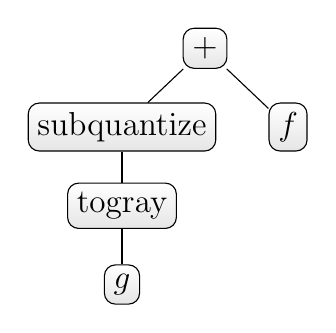
\begin{tikzpicture}[xscale=-1]
\tikzset{sibling distance=6em, level distance=1cm, font=\tt,
  every node/.style={font=\large, shape=rectangle, rounded corners, draw,
    align=center, top color=white, bottom color=gray!20}}

\node[grow=right] {$+$}
child { node {$f$} }
child { node {subquantize}
  child { node {togray}
    child { node {$g$} } } };

\end{tikzpicture}
\end{document}